\myChapter{Strumenti}
\section{Librerie software}
Il campo del Deep Learning è in costante e vertiginosa evoluzione. Ciò rende difficile, se non impossibile, essere aggiornati su ogni nuovo sviluppo del settore.

Al momento attuale le librerie software maggiormente diffuse sono \textit{TensorFlow} sviluppata da google, \textit{Torch} sviluppata da facebook, \textit{Theano} sviluppata dall'università di Montreal e \textit{Caffe} sviluppata dall'università di Berkeley. Senza scendere in ulteriori dettagli per le altre si prende in considerazione la più apprezzata (stando a GitHub), ovvero TensorFlow.
\section{TensorFlow} % (fold)
\label{sec:tensorflow}
Secondo la pagina ufficiale\cite{tensorflow}, TensorFlow è una libreria software open-source per il calcolo numerico tramite grafi di flussi di dati. I nodi di un grafo rappresentano operazioni matematiche, mentre gli archi rappresentano i tensori comunicanti fra loro. Può essere sfruttato in molti modelli di Machine Learning, al di là del Deep Learning. Uno dei vantaggi più importanti di TensorFlow, rispetto alle altre librerie, è che possiede un'architettura flessibile che permette agli sviluppatori di svolgere i calcoli su una o più CPU o GPU con una singola API.

L'estrema versatilità delle API, inoltre, facilita la possibilità di interfacciarsi a TensorFlow anche da parte di altre librerie, quali Keras.
% section tensorflow (end)
\subsection{Keras}
Secondo la pagina ufficiale\cite{keras}, Keras è una libreria di alto livello per sviluppare reti neurali, sviluppata da Fran\c{c}ois Chollet, scritta in Python ed in grado di interfacciarsi sia a TensorFlow che a Theano.

Questa libreria è stata sviluppata a seguito del progetto di ricerca noto come ONEIROS (Open-ended Neuro-Electronic Intelligent Robot Operating System), ed è da considerarsi indipendente da istituzioni, organizzazioni o compagnie. Si tratta probabilmente della più supportata ed utilizzata dopo TensorFlow. Le ragioni del successo di Keras sono molteplici: 
\begin{itemize}
	\item La modularità, la semplicità e l'estendibilità garantiscono la facilità d'uso e la rapidità della prototipazione.
	\item Supporta l'implementazione di reti ricorrenti e convoluzionali permettendo la combinazione fra di esse, inoltre è possibile definire layer personalizzati per integrare strutture complesse in una rete (ad esempio MDN).
	\item Come TensorFlow (appoggiandosi ad esso), può eseguire la computazione su CPU e/o GPU senza accorgimenti particolari.
\end{itemize}

\subsection{Recurrent Shop}
Secondo la documentazione\cite{recurrentshop}, Recurrent Shop è un framework adatto alla costruzione di reti ricorrenti complesse su Keras. Librerie come Keras permettono una facile prototipazione di layer e modelli tramite l'iterazione immediata fra implementazioni di architetture diverse. Esse presentano però alcune carenze nella definizione di reti ricorrenti personalizzate. Una delle più rilevanti è l'implementazione di celle ricorrenti riutilizzabili. In Keras, come in molte altre librerie, sono presenti layer (quali LSTM, GRU ecc...) che possono essere utilizzati solo così come vengono implementati, senza poterli sfruttare per includerli all'interno di una RNN complessa. A sua volta implementare la logica di una RNN in un layer personalizzato può risultare un'operazione onerosa, ad esempio informazioni riguardo gli stati (forma e inizializzazione) necessitano di essere aggiornate tramite metodi diversi \lstinline{get_initial_states} e \lstinline{reset_states}. Molte architetture presentano quindi implementazioni non banali, quali:
\begin{itemize}
	\item Sincronizzazione degli stati in tutti i layers di una pila di RNN.
	\item Readout, ovvero il passaggio dell'output di un layer di una pila di RNN come input del time step successivo.
	\item Decoder: RNN che vedono tutta la sequenza (o il vettore) di input ad ogni time step.
	\item \textit{Teacher forcing}: l'utilizzo del dato reale al tempo t-1 per la previsione al tempo t durante il training.
	\item RNN nidificate.
	\item Inizializzazione degli stati tramite distribuzioni diverse.
\end{itemize}

Recurrent Shop facilita l'implementazione di queste strutture, permettendo la scrittura di RNN di complessità arbitraria attraverso le API di Keras. In sostanza, è possibile costruire modelli standard di Keras, in cui vengano definite le logiche dei singoli time step, e convertirli in layer ricorrenti attraverso Recurrent Shop\footnote{Questa libreria è stata usata nel prototipo di riproduzione in Keras visibile in appendice.}.
\section{Dataset}
\label{sec:dataset}
\begin{table}[ht]\tiny
\centering
	\begin{tabular}{| c | c | c | c | c | c | c |}
		\hline
		alarm clock & ambulance & angel & ant & barn & basket & bee \\
		\hline
		bicycle & book & bridge & bulldozer & bus & butterfly & cactus \\
		\hline
		castle & cat & chair & couch & crab & cruise ship & dolphin \\
		\hline
		duck & elephant & eye & face & fan & fire hydrant & firetruck \\
		\hline
		flamingo & flower & garden & hand & hedgehog & helicopter & kangaroo \\
		\hline
		key & lighthouse & lion & map & mermaid & octopus & owl \\
		\hline
		paintbrush & palm tree & parrot & passport & peas & penguin & pig \\
		\hline
		pineapple & postcard & power outlet & rabbit & radio & rain & rhinoceros \\
		\hline
		roller coaster & sandwich & scorpion & sea turtle & sheep & skull & snail \\
		\hline
		snowflake & speedboat & spider & strawberry & swan & swing set & tennis racquet \\
		\hline
		& Monna Lisa & toothbrush & truck & whale & windmill & \\
		\hline
	\end{tabular}
	\caption{Le 75 classi inserite inizialmente in \texttt{QuickDraw}}
	\label{tab:1}
\end{table}
Come già citato nell'introduzione \ref{sec:prefazione}, \texttt{QuickDraw} è un dataset di immagini vettoriali ottenuti attraverso \textit{Quick, Draw!}\cite{quickdraw}, un gioco online dove agli utenti viene chiesto di disegnare oggetti appartenenti ad alcune classi entro 20 secondi. \texttt{QuickDraw} attualmente consiste di centinaia di categorie, ognuna delle quali è un dataset di almeno settantamila immagini di training e duemilacinquecento immagini di validazione e test, in tabella~\ref{tab:1} sono elencate le 75 classi che hanno costituito il nucleo iniziale del dataset. \textit{Quick, Draw!} continua a fornire dati quotidianamente e, di tanto in tanto, nuove tipologie di oggetti vengono aggiunte. Questo ha portato ad ampliare considerevolmente il volume di partenza, arrivando in alcune classi a più che raddoppiare il training set.

Le immagini nel dataset sono rappresentate in un formato che le codifica come sequenze di tratti di penna, detto \textit{stroke-3} \footnote{in estensione al formato utilizzato in \cite{sequence}.}. L'evento binario che rappresenta lo stato della penna è poi codificato come evento multi-stato, in un formato detto \textit{stroke-5}, attraverso lo \textit{one hot encoding} delle possibili configurazioni, prima di essere passato alla rete. Le coordinate assolute iniziali del disegno sono poste all'origine degli assi, lo schizzo è una lista di punti dove ogni punto è un vettore che consiste di 5 elementi: $(\Delta x, \Delta y, p_1, p_2, p_3)$. I primi due elementi sono le variazioni posizionali della penna, rispetto alla posizione precedente, in direzione x e y. I successivi tre elementi rappresentano la codifica dei possibili stati della penna: \textit{p\textsubscript{1}} indica che nell'arco dello spostamento definito dai primi due elementi la penna sarà poggiata sul foglio, \textit{p\textsubscript{2}} specifica invece che la penna è sollevata dal foglio nel punto corrente e perciò non traccerà alcuna linea. \textit{p\textsubscript{3}} infine indica che il disegno è concluso e che eventuali punti seguenti, compreso il corrente, non saranno considerati.

Dopo la codifica, i tratti vengono semplificati attraverso l'algoritmo \textit{Ramer-Douglas-Peucker}\cite{rdp}, che riduce il numero di punti necessari a visualizzare una determinata curva, con un parametro $\epsilon$ che è stato stabilito essere pari a 2. I dati originariamente sono salvati come immagini in pixel, la conversione in liste di punti viene poi ottenuta attraverso un fattore di scala, che è calcolato per imporre che la variazione standard delle distanze nel training set sia pari ad 1. Per comodità non è stato scelto di portare gli offset a media zero, dato che tipicamente le medie sono già relativamente piccole.
\begin{figure}[ht]
	\centering
	\includegraphics[width=\linewidth]{img/turtle_code.png}
	\caption{Uno sketch e la lista di tratti corrispondenti, in formato \textit{stroke-5}, i colori corrispondono all'ordine della sequenza.}
	\label{fig:1.18}
\end{figure}
\section{Modello} % (fold)
\label{sec:modello}
\begin{figure}[ht]
	\centering
	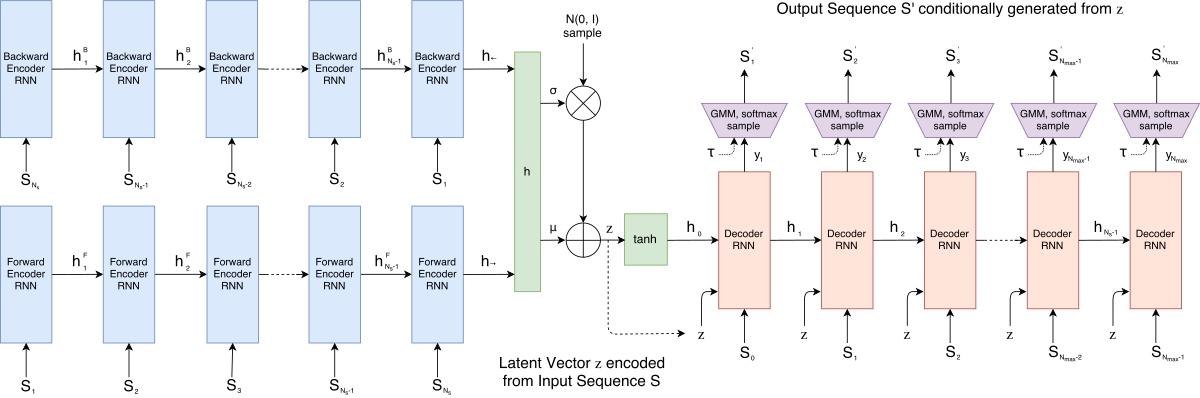
\includegraphics[width=\linewidth]{img/sketch_model.png}
	\caption{Sketch-rnn}
	\label{fig:1.15}
\end{figure}

In accordo a \cite{sketchrnn}, il modello di sketch-rnn è un VAE \ref{sec:vae} composto da reti ricorrenti \ref{sec:reti_ricorrenti}, che formano uno schema "molti a molti" \ref{enum:recurrence}. L'encoder è una RNN bidirezionale \ref{sub:reti_bidirezionali} che prende in input uno schizzo e come output genera un vettore di latenza di dimensione \textit{N\textsubscript{z}}. Nello specifico, secondo la definizione di rete bidirezionale, l'input\footnote{Si ricorda che ogni sketch in input non è altro che una tabella di sequenze di tratti.} viene passato alla rete anche invertito, dopodiché i due stati finali risultanti vengono concatenati in uno stato $\boldsymbol{h} = [\boldsymbol{h_\rightarrow} ; \boldsymbol{h_\leftarrow}]$. L'output $\boldsymbol{h}$ viene poi proiettato su due vettori, rispettivamente $\boldsymbol{\mu}$ e $\boldsymbol{\hat\sigma}$, entrambi di dimensione \textit{N\textsubscript{z}}, attraverso un layer densamente connesso \ref{sec:reti_densamente_connesse}. $\boldsymbol{\hat\sigma}$ viene convertito in un parametro di deviazione standard (non negativo) $\boldsymbol{\sigma}$ attraverso un'operazione esponenziale, $\boldsymbol{\mu}$ e $\boldsymbol{\sigma}$ vengono poi utilizzati, insieme a $\mathcal{N}(0, I)$, che è un vettore di variabili gaussiane identicamente distribuite di dimensione \textit{N\textsubscript{z}}, per costruire un vettore latente $\boldsymbol{z} \in \mathbb{R}^{N_z}$ \ref{sec:vae}:
\begin{equation}
	\label{repar_trick}
	\boldsymbol{\mu} = W_\mu \boldsymbol{h} + b_\mu, \boldsymbol{\hat\sigma} = W_{\hat\sigma} \boldsymbol{h} + b_{\hat\sigma}, \boldsymbol{\sigma} = \exp (\frac{\boldsymbol{\hat\sigma}}{2}), \boldsymbol{z} = \boldsymbol{\mu} + \boldsymbol{\sigma} \odot \mathcal{N}(0, I)
\end{equation}
Attraverso questo schema di codifica, il vettore di latenza $\boldsymbol{z}$ risulta essere una variabile casuale condizionata rispetto al disegno in input ($Q(\boldsymbol{z} | \boldsymbol{x})$).

Il decoder è una RNN (potenzialmente autoregressiva\footnote{L'output ad ogni time-step viene riportato come input per il time-step successivo.}) che genera in output degli schizzi condizionati ad un vettore latente $\boldsymbol{z}$ dato. Lo stato iniziale $\boldsymbol{h_0}$ e, se disponibile \ref{sub:lstm}, lo stato delle celle $\boldsymbol{c_0}$ del layer nel decoder vengono inizializzati da un layer densamente connesso, con una tangente iperbolica come funzione d'attivazione\footnote{Questo garantisce che i valori siano compresi fra -1 e 1.}: $[\boldsymbol{h_0} ; \boldsymbol{c_0}] = \tanh(W_z \boldsymbol{z} + b_z)$.
Ad ogni passo, il decoder prende in input il punto precedente \textit{S\textsubscript{i-1}} e il vettore di latenza $\boldsymbol{z}$, che vengono concatenati come un vettore $\boldsymbol{x}_i$, dove \textit{S\textsubscript{0}} è definito come $(0, 0, 1, 0, 0)$. L'output di ogni time-step è costituito dai parametri di una distribuzione di probabilità per il prossimo punto nei dati \textit{S\textsubscript{i}}.
\begin{equation}
	\label{gaussian_mixture}
	p(\Delta x, \Delta y) = \sum_{j=1}^M \Pi_j \mathcal{N}(\Delta x, \Delta y | \mu_{x,j}, \mu_{y,j}, \sigma_{x,j}, \sigma_{y,j}, \rho_{xy, j}), dove \sum_{j=1}^M \Pi_j = 1
\end{equation}

Nell'equazione \ref{gaussian_mixture} è mostrato come la rete modella $(\Delta x, \Delta y)$: attraverso un modello a mistura Gaussiana \ref{sec:mdn} (GMM - Gaussian mixture model), con \textit{M} distribuzioni normali \cite{gmm}. (\textit{q\textsubscript{1}}, \textit{q\textsubscript{2}}, \textit{q\textsubscript{3}}) invece, sono presi come distribuzione categorica allo scopo di modellare i dati reali (\textit{p\textsubscript{1}}, \textit{p\textsubscript{2}}, \textit{p\textsubscript{3}}), dove (\textit{q\textsubscript{1}} + \textit{q\textsubscript{2}} + \textit{q\textsubscript{3}} = 1)\footnote{Come in \cite{fake_chinese} e \cite{draw_chinese}.}\footnote{Si ricorda che la sequenza generata è condizionata ad una variabile latente $\boldsymbol{z}$ campionata dall'encoder.}.

$\mathcal{N}(\Delta x, \Delta y | \mu_{x,j}, \mu_{y,j}, \sigma_{x,j}, \sigma_{y,j}, \rho_{xy, j})$ è la funzione di distribuzione di probabilità per una distribuzione normale bivariata. Ognuna delle M distribuzioni normali bivariate consiste di cinque parametri: $(\mu_{x}, \mu_{y}, \sigma_{x}, \sigma_{y}, \rho_{xy})$ dove $\mu_{x}, \mu_{y}$ sono le medie, $\sigma_{x}, \sigma_{y}$ sono le deviazioni standard e $\rho_{xy}$ è il corrispondente parametro di correlazione. Il vettore $\Pi$ di lunghezza \textit{M}, a sua volta considerato come una distribuzione categorica, corrisponde ai pesi delle distribuzioni nel GMM. Come conseguenza di questa struttura, si deduce che l'output del decoder debba avere dimensione $5M + M + 3.$\footnote{dove il primo termine indica i parametri di ogni distribuzione, il secondo la lunghezza di $\Pi$ e il terzo corrisponde ai logit per generare (\textit{q\textsubscript{1}}, \textit{q\textsubscript{2}}, \textit{q\textsubscript{3}})}

Il successivo hidden state della RNN nel decoder, è proiettato nel vettore di output $y_i$ attraverso uno strato densamente connesso:
\begin{equation}
	\label{output}
	x_i = [S_{i-1} ; \boldsymbol{z}], [h_i ; c_i] = forward(x_i, [h_{i-1} ; c_{i-1}]), y_i = W_y h_i + b_y, y \in \mathbb{R}^{6M + 3}
\end{equation}
Il vettore $y_i$ è poi suddiviso nei parametri della distribuzione di probabilità per il prossimo punto nei dati:
\begin{equation}
	\label{parameters}
	[(\hat\Pi_1, \mu_{x}, \mu_{y}, \hat\sigma_{x}, \hat\sigma_{y}, \hat\rho_{xy})_1, ..., (\hat\Pi_M, \mu_{x}, \mu_{y}, \hat\sigma_{x}, \hat\sigma_{y}, \hat\rho_{xy})_M(\hat{q}_1, \hat{q}_2), \hat{q}_3)] = y_i
\end{equation}
Per assicurarsi che la deviazione standard non risulti negativa e che il valore di correlazione sia nell'intorno (-1, 1), si applicano gli operatori esponenziali ai $\hat\sigma$ e tangente iperbolica ai $\hat\rho$:
\begin{equation}
	\label{exp}
	\sigma_x = \exp(\hat\sigma_x), \sigma_y = \exp(\hat\sigma_y) \implies \sigma_x, \sigma_y > 0
\end{equation}
\begin{equation}
	\label{tanh}
	\rho_xy = \tanh(\hat\rho_xy) \implies \rho_xy \in (-1, 1)
\end{equation}
Le probabilità per le distribuzioni categoriche, invece, sono calcolate attraverso un'operazione di \textit{softmax}:
\begin{equation}
	\label{softmax_q}
	q_k = \frac{\exp(\hat q_k)}{\sum_{j=1}^3\exp(\hat q_j)}, k \in {1, 2, 3}, \implies q_k \in (0, 1), \sum_j q_k = 1
\end{equation}
\begin{equation}
	\label{softmax_p}
	\Pi_k = \frac{\exp(\hat\Pi_k)}{\sum_{j=1}^M\exp(\hat\Pi_j)}, k \in {1, ..., M} \implies \Pi_k \in (0, 1), \sum_j \Pi_k = 1
\end{equation}
\begin{minipage}{\linewidth}
\begin{lstlisting}[language = Python, frame = single, caption = {Implementazione in Keras del metodo per l'estrazione e la normalizzazione dei parametri della distribuzione}, captionpos = b]
def get_mixture_coef(output):
    out_pi = output[:, :20]
    out_mu_x = output[:, 20:40]
    out_mu_y = output[:, 40:60]
    out_sigma_x = output[:, 60:80]
    out_sigma_y = output[:, 80:100]
    out_ro = output[:, 100:120]
    pen_logits = output[:, 120:123]
    # use softmax to normalize pi and q into prob distribution
    out_pi = K.exp(out_pi)
    normalize_pi = 1 / (K.sum(out_pi, axis=1, keepdims=True))
    out_pi = normalize_pi * out_pi
    out_q = K.exp(pen_logits)
    normalize_q = 1 / (K.sum(out_q, axis = 1, keepdims = True))
    out_q = normalize_q * out_q
    out_ro = K.tanh(out_ro)
    # use exponential to make sure sigma is positive
    out_sigma_x = K.exp(out_sigma_x)
    out_sigma_y = K.exp(out_sigma_y)
    return out_pi, out_mu_x, out_mu_y, out_sigma_x, out_sigma_y, out_ro, pen_logits, out_q
\end{lstlisting}
\end{minipage}
Una volta ottenuti i parametri appropriati, diventa possibile calcolare le distribuzioni normali bivariate, tramite:
\begin{equation}
	\label{bivariate}
	\mathcal{N}(\Delta x, \Delta y | \mu_{x}, \mu_{y}, \sigma_{x}, \sigma_{y}, \rho_{xy}) = \frac{\exp(\frac{-Z}{2(1-\rho_{xy}^2)})}{2\pi\sigma_{x}\sigma_{y}\sqrt{1-(\rho_{xy})^2}}
\end{equation}
con:
\begin{equation}
	\label{z}
	Z = \frac{(\Delta x - \mu_x)^2}{\sigma_x^2} + \frac{(\Delta y - \mu_y)^2}{\sigma_y^2} - \frac{\rho_{xy}((\Delta x - \mu_x)(\Delta y - \mu_y))}{\sigma_x\sigma_y}
\end{equation}
\begin{minipage}{\linewidth}
\begin{lstlisting}[language = Python, frame = single, caption = {Implementazione in Keras del calcolo della normale bivariata}, captionpos = b]
def tf_bi_normal(x, y, mu_x, mu_y, sigma_x, sigma_y, ro):
    norm1 = x_ - mu_x
    norm2 = y_ - mu_y
    sigma = sigma_x * sigma_y
    z = (K.square(norm1 / (sigma_x + 1e-8)) + K.square(norm2 / (sigma_y + 1e-8)) - (2 *
         ro * norm1 * norm2) / (sigma + 1e-8) + 1e-8)
    ro_opp = 1 - K.square(ro)
    result = K.exp(-z / (2 * ro_opp + 1e-8))
    denom = 2 * np.pi * sigma * K.square(ro_opp) + 1e-8
    result = result / denom + 1e-8
    return result
\end{lstlisting}
\end{minipage}
Sempre in accordo a \cite{sketchrnn}, un problema chiave dell'apprendimento sta nello stabilire quando il modello debba smettere di disegnare. Le probabilità dei tre tipi di tratto \footnote{Rispettivamente: penna sul foglio, penna sollevata e fine del disegno.} sono molto sbilanciate e ciò rende il modello difficile da addestrare. La probabilità di un evento \textit{p\textsubscript{1}} sono molto più alte di quelle di un evento \textit{p\textsubscript{2}} e l'evento \textit{p\textsubscript{3}} avviene una volta sola per disegno. L'approccio seguito in alcuni lavori\footnote{Vedere \cite{fake_chinese} e \cite{draw_chinese}.} è stato quello di pesare differentemente ogni evento della penna nel calcolo dell'errore, ad esempio imponendo manualmente i valori (1, 10, 100). In sketch-rnn è stato scelto un approccio più robusto e funzionale: tutte le sequenze sono generate dal modello fino ad \textit{N\textsubscript{max}}, che è la lunghezza del disegno più lungo del training set. Dato che la lunghezza del generico sketch \textit{S} è tipicamente minore di \textit{N\textsubscript{max}}, \textit{S\textsubscript{i}} è impostato a (0, 0, 0, 0, 1) per ogni \textit{i} > \textit{N\textsubscript{s}}\ref{sec:dataset}.

Dopo il training è possibile campionare disegni dal modello, questo procedimento è effettuato utilizzando il decoder in modo autoregressivo: ad ogni time-step vengono generati i parametri sia del GMM che della distribuzione categorica tramite i quali si ricava un punto \textit{S'\textsubscript{i}}, questo viene poi concatenato all'input\footnote{Una variabile casuale di dimensione \textit{N\textsubscript{z}}.} del time step seguente. Il procedimento prosegue finché \textit{p\textsubscript{3}} = 1 o quando viene raggiunto \textit{i} = \textit{N\textsubscript{max}}.

Come per l'encoder, l'output ottenuto in questo modo non è deterministico, si tratta di una sequenza casuale condizionata rispetto al vettore di latenza. Il livello di casualità puà essere controllato introducendo un parametro di temperatura $\tau$:
\begin{equation}
	\label{temperature}
	\hat q_k \rightarrow \frac{\hat q_k}{\tau}, \hat \Pi_k \rightarrow \frac{\hat \Pi_k}{\tau}, \sigma_x^2 \rightarrow \sigma_x^2 \tau, \sigma_y^2 \rightarrow \sigma_y^2 \tau
\end{equation}
Questo valore può essere utilizzato sui parametri delle softmax della distribuzione categorica e sulle deviazioni standard della normale bivariata. Il parametro è tipicamente scelto fra 0 e 1, nel caso in cui $\tau = 0$ il modello diventa deterministico e i punti generati risulteranno essere i punti più probabili della funzione di densità di probabilità.
% section modello (end)
\subsection{training} % (fold)
\label{sub:training}
La procedura di training segue l'approccio di un VAE \cite{VAE}, dove la funzione di loss è composta dalla somma di due termini: \textit{Reconstruction Loss} (l'errore di ricostruzione), \textit{L\textsubscript{R}}, e la divergenza di Kullback-Leibler, \textit{L\textsubscript{KL}}. Il termine dell'errore di ricostruzione \ref{rec_loss} massimizza la verosimiglianza logaritmica della distribuzione di probabilità generata dalla rete, nel descrivere l'oggetto di training S. Si può calcolare l'errore di ricostruzione utilizzando i parametri generati dalla PDF e il dato di training, in questo modo otteniamo una descrizione dell'errore attraverso due componenti: la somma del logaritmo degli errori sui termini di distanza, \textit{L\textsubscript{s}} \ref{rec_loss_s}, e la somma logaritmica degli errori sugli stati della penna $(p_1, p_2, p_3)$, \textit{L\textsubscript{p}} \ref{rec_loss_p}
\begin{equation}
	\label{rec_loss_s}
	L_s = - \frac{1}{N_{max}}\sum_{i=1}^{N_s}\log(\sum_{j=1}^M \Pi_{j,i} \mathcal{N}(\Delta x_i, \Delta y_i | \mu_{x,j, i}, \mu_{y,j, i}, \sigma_{x,j, i}, \sigma_{y,j, i}, \rho_{xy, j, i}))
\end{equation}
\begin{equation}
	\label{rec_loss_p}
	L_p = - \frac{1}{N_{max}}\sum_{i=1}^{N_{max}}\sum_{k=1}^{3} p_{k, i}\log(q_{k, i})
\end{equation}
\begin{equation}
	\label{rec_loss}
	L_R = L_s + L_p
\end{equation}

Si noti che nel calcolo della sommatoria sull'errore di offset l'indice si ferma a \textit{N\textsubscript{S}} scartando tutti i valori successivi mentre, \textit{L\textsubscript{p}} è calcolata usando tutti i parametri che modellano $(p_1, p_2, p_3)$ fino a \textit{N\textsubscript{max}}. Questo metodo di calcolo della perdita risulta più robusto e permette al modello di apprendere quando smettere di disegnare, a differenza del metodo citato precedentemente che suggerisce di soppesare diversamente i valori $p_i$ \ref{sec:modello}.

\begin{minipage}{\linewidth}
\begin{lstlisting}[language = Python, frame = single, caption = {Implementazione in Keras del calcolo dell'errore di ricostruzione, suddiviso fra i termini dell'errore nell'offset $(L_s)$ e l'errore degli stati della penna $(L_p)$}, captionpos = b]
def get_lossfunc(out_pi, out_mu_x, out_mu_y, out_sigma_x, out_sigma_y, out_ro, out_q, x, y, logits):
    # L_r loss term calculation, L_s part
    result = tf_bi_normal(x, y, out_mu_x, out_mu_y, out_sigma_x, out_sigma_y, out_ro)
    result = result * out_pi
    result = K.sum(result, axis=1, keepdims=True)
    result = -K.log(result + 1e-8)
    fs = 1.0 - logits[:, 2]
    fs = K.reshape(fs, (-1, 1))
    result = result * fs
    # L_r loss term, L_p part
    result1 = K.categorical_crossentropy(out_q, logits, from_logits = True)
    result1 = K.reshape(result1, (-1, 1))
    result = result + result1
    return K.mean(result)
\end{lstlisting}
\end{minipage}

Il termine di loss della divergenza KL misura la differenza fra la distribuzione del vettore latente $\boldsymbol{z}$ e un vettore di distrubizioni Gaussiane IID con media zero e varianza unitaria. Ottimizzare secondo questo termine permette di minimizzare questa differenza. Sempre secondo i risultati di \cite{VAE}:
\begin{equation}
	\label{KL}
	L_{KL} = - \frac{1}{2N_z}(1 + \boldsymbol{\hat\sigma} - \boldsymbol{\mu}^2 - \exp(\boldsymbol{\hat\sigma}))
\end{equation}
La funzione di loss complessiva non è altro che la somma pesata dei sopracitati termini $L_R$ e $L_{KL}$, ovvero:
\begin{equation}
	\label{loss}
	Loss = L_R + w_{KL}L_{KL}
\end{equation}

Esiste un compromesso fra l'ottimizzare secondo un termine rispetto all'altro: per $w_{KL} \rightarrow 0$, il modello si avvicina a quello di un autoencoder puro, sacrificando l'abilità di forzare una distribuzione a priori sullo spazio di latenza, ottenendo migliori risultati nella ricostruzione. Si noti che nella generazione non condizionale, dove il modello è costituito dal solo decoder, non sarà presente il termine $L_{KL}$.
\begin{figure}
	\centering
	\includegraphics[width=\textwidth]{img/tradeoff_loss.png}
	\caption{Compromesso fra $L_R$ e $L_{KL}$, su due modelli addestrati su dataset con singola classe(sinistra). Il grafo della \textit{Validation Loss} per modelli addestrati sulla classe Yoga, al variare del peso $w_{KL}$, da \cite{sketchrnn}}
	\label{fig:1.19}
\end{figure}
In fig. \ref{fig:1.19} è illustrato il compromesso, ottenuto al variare di $w_{KL}$, fra l'errore di ricostruzione e la divergenza KL sul test set, confrontato (a destra) con un modello costituito dal solo decoder. Dato che un modello non condizionale non riceve informazioni precedenti riguardo al disegno che deve generare, la metrica $L_R$ dei modelli a decoder è utilizzata come limite superiore per i modelli condizionali a variabile latente.
% subsection training (end)